\section{Del og Hersk}
\hrulefill
\begin{itemize}
\item De 3 trin
  \begin{itemize}
  \item Del
  \item Hersk
  \item Foren
  \end{itemize}
\item Merge-sort
  \begin{itemize}
  \item Merge
  \item Merge-sort
  \end{itemize}
\item Rekursionsligninger
\item Rekurstionstræer
\item Substitutions metoden
  \begin{itemize}
  \item Lav et gæt
  \item Bevis gættet med matematisk induktion
  \end{itemize}
\item Master metoden
  \begin{itemize}
  \item De 3 tilfælde
  \item Hvornår den ikke kan bruges
  \end{itemize}
\item Tætteste par af punkter
\item Bevis for nedre grænse for sortering
\end{itemize}

\newpage
\subsection{De 3 trin}
Del og hersk er et algoritme paradigme, der løser problemer ved at følge 3 trin:\\
\begin{itemize}
\item \textbf{Del} problemet op i mindre underproblemer.
\item \textbf{Hersk} - løs de mindre underproblemer.
\item \textbf{Foren} de løste underproblemer til en løsning på de oprindelige problem
\end{itemize}

En del og hersk algoritme deler ofte problemet op rekursivt indtil den når et base case. 

\subsubsection{Merge-sort}
Merge-sort er en sorterings algoritmen der gør brug af del og hersk paradigmet for at sortere. Dens 3 trin er:
\begin{itemize}
\item Del et array op i midten så du har 2 arrays der skal sorteres.
\item Bliv ved med at dele til hvert array består af 1 element. Voila! Dette array er nu trivielt sorteret.
\item Foren 2 sorterede arrays til 1 array, således at det nye array også er sorteret.
\end{itemize}

Merge-sort gør brug af en vigtig hjælpefunktion \textbf{merge}. Merge funktionen forener 2 arrays sådan at de er sorterede efter forening.

\begin{algorithm}[H]
  \caption{Merge hjælpe funktionen}
  \begin{algorithmic}[1]
    \State $A[p..q..r] \gets$ Delarray der skal sorteres  
    \Function{MERGE}{$A, p, q, r$}
    \State $n_1 = q - p + 1$
    \State $n_2 = r - q$
    \State $left[1 .. n_1 + 1]$
    \State $right[1 .. n_2 + 1]$
    \For{$i=1$ \textbf{ to } $n_1$}
    \State $left[i] = A[p + i - 1]$ \Comment{Fylder $left$ med venstre delarray}
    \EndFor
    \For{$i=1$ \textbf{ to } $n_2$}
    \State $right[i] = A[q + j]$ \Comment{Fylder $right$ med højre delarray}
    \EndFor
    \State $left[n_1 + 1] = \infty$
    \State $right[n_2 + 1] = \infty$ \Comment{Sætter sentinel værdier for enden}
    \State $i = 1$
    \State $j = 1$
    \For{$k=p$ \textbf{ to } $p$}
    \If{$left[i] \leq right[j]$}
    \State $A[k] = left[i]$
    \State $i = i + 1$
    \Else
    \State $A[k] = right[j]$
    \State $j = j + 1$
    \EndIf
    \EndFor
    \EndFunction
  \end{algorithmic}
\end{algorithm}

Merge funktionen har en køretid på $\O(n)$

Selve Merge-sort funktionen er meget simpel.
\begin{algorithm}[H]
  \caption{Merge-sort funktionen}
  \begin{algorithmic}[1]
    \State $A[p..q] \gets$ Delarray der skal sorteres  
    \Function{MERGE-SORT}{$A, p, q$}
    \If{$p < r$}
    \State $q = \lfloor \frac{p + r}{2} \rfloor$
    \State MERGE-SORT($A, p, q$)
    \State MERGE-SORT($A, q + 1, r$)
    \State MERGE($A, p, q, r$)
    \EndIf
    \EndFunction
  \end{algorithmic}
\end{algorithm}

\subsection{Rekursionsligninger}
For at beskrive del og hersk algoritmers køretid, skal vi have en måde at beskrive rekursive funktioners køretid. Dette gøres med rekursionsligninger. Hvis vi kigger på merge-sorts køretid $T(n)$, så ser vi, at den splitter arrayet op i to stykker som den rekursivt kalder merge-sort på, det giver $T(n) = T(\lfloor \frac{n}{2} \rfloor) + T(\lceil \frac{n}{2} \rceil)$, det viser sig at vi kan fjerne floor og ceil funktionerne da de ikke ændre køretiden asymptotisk, så vi får $T(n) = 2T(\frac{n}{2})$. Vi skal også huske, at merge-sort kalder merge funktionen i hvert rekursive kald, hvilket lægger $cn$ til hvert rekursive kald, hvor $c$ beskriver de konstanter i merges køretid. Så den endelige rekursionsligning for merge-sort bliver
$$T(n) = 2T(\frac{n}{2}) + cn$$
\subsection{Rekursionstræer}
I nogle tilfælde, når man skal beskrive rekursionligninger asymptotisk, kan det være meget nyttigt at tegne et rekursionstræ, der viser per-level-cost af hvert rekursionskald, og hvor dybt rekursionskaldene går. Rekursionstræet for merge-sort ses på figur 1.

\begin{figure}[h!]
  \caption{Rekursionstræ for merge-sort $T(n) = 2T(\frac{n}{2}) + cn$}
%\begin{center}
  \begin{equation*}
    \O(\log_2(n))\left \{
      \begin{gathered}
        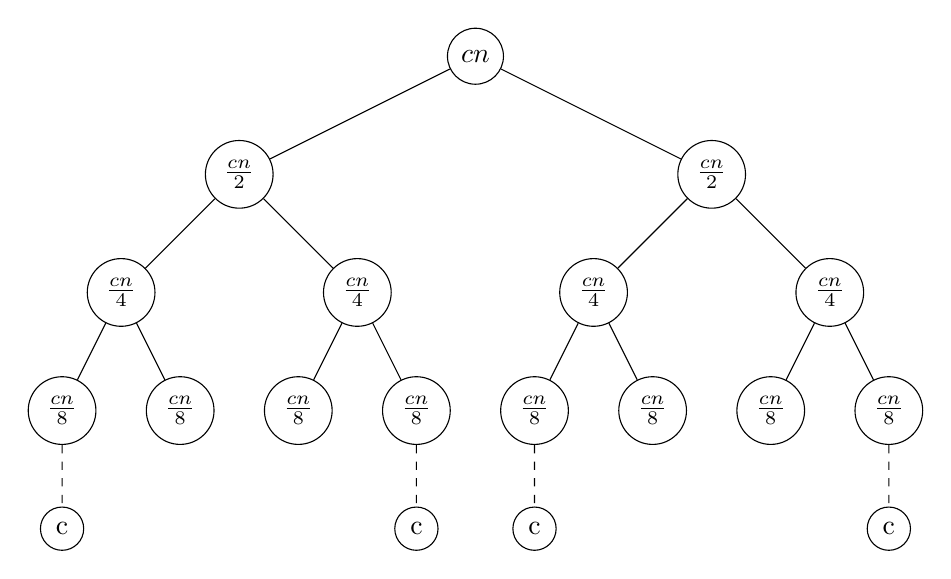
\begin{tikzpicture}[every node/.style = {shape=circle, draw, align=center}, level distance=1.5cm,
          level 1/.style={sibling distance=6cm},
          level 2/.style={sibling distance=3cm},
          level 3/.style={sibling distance=1.5cm},
          emph/.style={edge from parent/.style={dashed,draw}}]
          % Definer en knude \node(label til knude)[label=vinkel omkring center af knude :tekst på label] {tekst i knude}
          \node(A) at (0, 0) {$cn$}
          % Definer et barn til en knude child { node[label=vinkel omkring center af knude :tekst på label]  {navn på knude}}
          child { node {$\frac{cn}{2}$}
            child { node {$\frac{cn}{4}$}
              child { node {$\frac{cn}{8}$}
                child[emph] { node {c} }}
              child { node {$\frac{cn}{8}$} }}
            child { node {$\frac{cn}{4}$}
              child { node {$\frac{cn}{8}$} }
              child { node {$\frac{cn}{8}$}
                child[emph] { node {c} }}}}
          child { node {$\frac{cn}{2}$}
            child { node {$\frac{cn}{4}$}
              child { node {$\frac{cn}{8}$}
                child[emph] { node {c} }}
              child { node {$\frac{cn}{8}$} }}
            child { node {$\frac{cn}{4}$}
              child { node {$\frac{cn}{8}$} }
              child { node {$\frac{cn}{8}$}
                child[emph] { node {c} }}}};
        \end{tikzpicture}
      \end{gathered}
    \right.
  \end{equation*}
%\end{center}
\end{figure}

For bestemme køretiden ud fra rekursionstræet summeres alle per-level-costs for rekursionslagene. Hver lags cost summeres til $cn$, hvilket er $\O(n)$, og fordi $n$ halveres hver gang er træet $\log_2(n)$ dybt. Køretiden er derfor $\O(n\log_2(n))$. For at være mere grundig i sin argumentation, kan man bruge substitutionsmetoden efter man har lavet sit rekursionstræ.
\subsection{Substitutionsmetoden}
Substitutionsmetoden er en anden måde at analysere rekursionsligninger. Substitutionsmetoden består af to trin
\begin{itemize}
\item Lav et gæt $f(n)$. Lav evt. et rekursionstræ for at få en fornemmelse af rekursionsligningens køretid.
\item Bevis at gættet er korrekt. Her bruges matematisk induktion til at vise at rekursionsligningen er $T(n) = \O(f(n))$, ved at antage $T(m) \leq cf(m), m < n$ og derefter vise $T(n) \leq cf(n)$.
\end{itemize}

I tilfældet med merge-sort, skal vi bevise at $T(n) = Ø(nlgn)$, som er vores gæt ud fra rekursionstræet:\\

\begin{proof}
  Vi antager at $T(m) \leq cmlgm$:
  \begin{align*}
    T(n) &= 2T(\frac{n}{2}) + n \leq cnlgn\\
         &= 2(c\frac{n}{2}lg\frac{n}{2}) + n \leq cnlgn\\
         &= 2(\frac{cnlg2}{2} - \frac{cn}{2}) + n \leq cnlgn\\
         &= cnlgn - cn + n \leq cnlgn
  \end{align*}
  $cnlgn - cn + n \leq cnlgn$ gælder for alle $c \geq 1$
\end{proof}

\subsection{Master metoden}
I Master metoden tager man udgangspunkt i rekursionsligninger med formen
$$T(n) = aT(\frac{n}{b}) + f(n)$$

og sammenligner dem med $n^{\log_b(a)}$. Rekursionsligningen beskriver at vi vi deler vores problem op i $a$ bidder, hver af størrelse $\frac{n}{b}$, og hvor tiden for de ikke-rekursive kald er $f(n)$.\\

Der er tre tilfælde i master method, som beskrives i \textbf{master theorem}
\begin{theorem}
  Lad $a \geq 1$ og $b \geq 1$ være konstanter. Lad $f(n)$ være en asymptotisk positiv funktion. Lad $T(n) = aT(\frac{n}{b}) + f(n)$ være en rekursionsligning på de positive heltal, og hvor $\frac{n}{b}$ kan betyde både $\lfloor \frac{n}{b}\rfloor$ og $\lceil \frac{n}{b}\rceil$.\\
  Så har $T(n)$ følgende asymptotiske grænser:
  \begin{enumerate}
  \item hvis $f(n) = \O(n^{\log_b(a) - \epsilon})$ for $\epsilon > 0$, så er $T(n) = \Theta(n^{\log_b(a)})$
  \item hvis $f(n) = \Theta(n^{\log_b(a)})$, så er $T(n) = \Theta(n^{\log_b(a)}lgn)$
  \item hvis $f(n) = \Omega(n^{\log_b(a) + \epsilon})$ for $\epsilon > 0$, så er $T(n) = \Theta(f(n))$
  \end{enumerate}
\end{theorem}

Hvis vi bruger master metoden på merge-sort, ser vi at vi har $a = 2, b=2, f(n)=n$, og vi kan sammenligne rekursionsligningen med $n^{\log_b(a)}$:
$$n = \Theta(n^{\log_2(2)}) \Rightarrow f(n) = n = \Theta(nlgn)$$

master method virker kun i de tilfælde hvor $f(n)$ enten er polynomisk større, i 1. tilfælde, og polynomisk mindre, i 3. tilfælde, end $n^{\log_b(a)}$. Det er grunden til at vi inkluderer en konstant $\epsilon > 0$
\subsection{Tætteste par af punkter}
Et andet problem der løses med del og hersk, er problemet med at finde det tætteste par af punkter. Givet en mængde punkter $Q$ med $n > \geq 2$ punkter skal vi finde to punkter $p_1 = (x_1, y_1)$ og $p_2 = (x_2, y_2)$ der har den mindste Euklidiske afstand $d(p_1, p_2) = \sqrt{(x_2 - x_1)^2 + (y_2 - y_1)^2}$. Den naive måde at løse problemet på, er ved at se på alle $(n \choose 2) = \Theta(n^2)$ punkter, og returnerer dem med lavest afstand.\\

Del og hersk algoritmen har rekursionsligning magen til merge-sort -- $T(n)=2T(\frac{n}{2}) + Ø(n) = Ø(nlgn)$. Hvert rekursive kald tager som argumenter en delmængde $P \subset Q$, arrays $X,Y$ som hver indeholder henholdsvis punkterne i $P$ sorteret efter stigende $x$-koordinat, og stigende $y$-koordinat. De 3 trin i del og hersk er for denne algoritme
\begin{itemize}
\item \textbf{Del}: Rekursivt del $P$ på en vertikal linje $l$ så vi har $|P_L| = \lfloor \frac{|P|}{2}\rfloor$ og $|P_R| = \lceil \frac{|P|}{2}\rceil$. Vi deler også $X$ og $Y$ op og sorterer delarrays, så vi får $X_L, X_R$ og $Y_L,Y_r$. Vi stopper de rekursive kald, når $|P| \leq 3$, hvorefter vi bruger den naive måde.
\item \textbf{Hersk}. Vi prøver at finde de tætteste par af punkter $\delta_L$ i $P_L$ og $\delta_R$ i $P_R$, og vi lader $\delta = min(\delta_L, \delta_R)$.
\item \textbf{Foren}: Det tætteste par af punkter er enten begge i $P_L$ eller begge i $P_R$, hvor $\delta$ så er den korteste afstand. Det er også muligt at det tætteste par af punkter, er et punkt $p_L \in P_L$ og $p_R \in P_R$, og algoritmen må tjekke for dette tilfælde.\\

  Hvis $p_L$ og $p_R$ er de tætteste par af punkter, så må de være indenfor et område der stikker $\delta$ ud fra $l$ på begge sider. For at finde tætteste par af punkter inden for dette vertikale område gør vi følgende:
  \begin{enumerate}
  \item Lad $Y'$ være alle de punkter inden for det vertikale område, sorteret efter stigende $y$-koordinat.
  \item For hvert punkt $p \in Y'$ tjek de næste 7 punkter efter $p$, og hold øje med den korteste afstand $\delta'$ til disse punkter.
  \item Hvis $\delta' < \delta$ så returner $\delta'$, ellers returner $\delta$. I begge tilfælde returnerer vi også de to tætteste punkter.
  \end{enumerate}
\end{itemize}

\textbf{Korrekthed}:\\
Det er let at se hvordan den vælger $\delta$, så det vi skal vise for at vise korrekthed, er hvordan vi finder $\delta'$. Vi vil nu bevise hvorfor vi kun skal tjekke afstanden mellem punkt $p \in Y'$ og de 7 næste punkter i $Y'$.\\
\begin{proof}
  Vi antager at den korteste afstand efter en forening, er mellem punkterne $p_L \in P_L$ og $p_R \in P_R$ med afstand $\delta' < \delta$. Siden de befinder sig i det vertikale område, må de være inden for en afstand af $\delta$ i deres vertikale afstand, og inden for en afstand af $\delta$ til $l$. Dette giver et $\delta \times 2\delta$ rektangel som de kan befinde sig i.\\
  
  Vi viser nu hvorfor der højst kan være 8 punkter i sådan et rektangel. Hvis vi den ene halvdel af rektanglet, den side der er i $P_L$, har vi et kvadrat med sidelængder $\delta$. Det højeste antal punkter vi kan have i det kvadrat, med sidelængder ikke mindre end $\delta$, er 4; et i hvert hjørne. Hvis vi antager at der er et 5. punkt i kvadratet, så må det ligge et sted, hvor dets afstand til et af de andre punkter er mindre end $\delta$, hvilket vil betyde at den korteste afstand ikke er mellem $p_L$ og $p_R$, men mellem to punkter i $P_L$. Det samme gør sig gældende i kvadratet i $p_R$. Der er 4 punkter som ligger på linjen $l$ -- to af hjørnerne i $P_L$ og to i $P_R$. Siden $Y'$ er sorteret, behøver vi kun tjekke de 7 punkter efter et givet punkt, for at finde det tætteste.
\end{proof}

For at opnå en køretid på $Ø(nlgn)$ \textbf{præsorterer} vi $X$, og $Y$, før det første rekursive kald, og i hvert rekursive kald, splitter vi dem i en \emph{omvendt} \texttt{MERGE}, der splitter dem i $X_L, X_R$ og $Y_L, Y_R$ således, at de splittede arrays stadig er sorterede, hvilket tager $Ø(n)$ tid. Da vi laver rekursive kald på $|P_L| = \lfloor \frac{|P|}{2}\rfloor$ og $|P_R| = \lceil \frac{|P|}{2}\rceil$, er det let at se rekursionsligningen $T(n) = 2T(\frac{n}{2}) + Ø(n) = Ø(nlgn)$.

\subsection{Bevis for nedre grænse for sortering}
Vi har brugt merge-sort som har en køretid på $Ø(nlgn)$, som vores eksempel, og det kan vises at den køretid er så god som det kan blive for sammenligningssorteringer.\\

Vi tager udgangspunkt i et \textbf{decision-tree}, hvor en knude repræsenter en sammenligning mellem to elementer $i:j$ i listen der skal sorteres. Hvis man går til venstre bytter man hvis $i \leq j$, og til højre bytter man når $i < j$.
\begin{theorem}
  Enhver sammenligningssorteringsalgoritme er $\Omega(nlgn)$.
\end{theorem}

\begin{proof}
  Der er $n!$ permutationer af listen og alle knuderne repræsenterer en forskellig permutation. En sortering svarer derfor til at tage nogle beslutninger i vores decision-tree indtil man ender i den permutation der er den sorterede, og vi skal derfor finde højden $h$ for at finde hvor mange trin algoritmen skal tage.\\

  Vi ved vi har med et fuldt binært træ, derfor er der højst $2^h$ blade, og vi har altså
  $$n! \leq 2^h$$

  Og vi finder højden ved at tage logaritmen
  $$lg(n!) \leq h$$

  $n! = \Theta(n^n)$ og vi har derfor

  $$nlgn \leq h$$

  Ergo er $h = \Omega(nlgn)$.
\end{proof}

%%% Local Variables:
%%% mode: latex
%%% TeX-master: "master"
%%% End:
